\documentclass{article}\usepackage[]{graphicx}\usepackage[]{color}
%% maxwidth is the original width if it is less than linewidth
%% otherwise use linewidth (to make sure the graphics do not exceed the margin)
\makeatletter
\def\maxwidth{ %
  \ifdim\Gin@nat@width>\linewidth
    \linewidth
  \else
    \Gin@nat@width
  \fi
}
\makeatother

\definecolor{fgcolor}{rgb}{0.345, 0.345, 0.345}
\newcommand{\hlnum}[1]{\textcolor[rgb]{0.686,0.059,0.569}{#1}}%
\newcommand{\hlstr}[1]{\textcolor[rgb]{0.192,0.494,0.8}{#1}}%
\newcommand{\hlcom}[1]{\textcolor[rgb]{0.678,0.584,0.686}{\textit{#1}}}%
\newcommand{\hlopt}[1]{\textcolor[rgb]{0,0,0}{#1}}%
\newcommand{\hlstd}[1]{\textcolor[rgb]{0.345,0.345,0.345}{#1}}%
\newcommand{\hlkwa}[1]{\textcolor[rgb]{0.161,0.373,0.58}{\textbf{#1}}}%
\newcommand{\hlkwb}[1]{\textcolor[rgb]{0.69,0.353,0.396}{#1}}%
\newcommand{\hlkwc}[1]{\textcolor[rgb]{0.333,0.667,0.333}{#1}}%
\newcommand{\hlkwd}[1]{\textcolor[rgb]{0.737,0.353,0.396}{\textbf{#1}}}%

\usepackage{framed}
\makeatletter
\newenvironment{kframe}{%
 \def\at@end@of@kframe{}%
 \ifinner\ifhmode%
  \def\at@end@of@kframe{\end{minipage}}%
  \begin{minipage}{\columnwidth}%
 \fi\fi%
 \def\FrameCommand##1{\hskip\@totalleftmargin \hskip-\fboxsep
 \colorbox{shadecolor}{##1}\hskip-\fboxsep
     % There is no \\@totalrightmargin, so:
     \hskip-\linewidth \hskip-\@totalleftmargin \hskip\columnwidth}%
 \MakeFramed {\advance\hsize-\width
   \@totalleftmargin\z@ \linewidth\hsize
   \@setminipage}}%
 {\par\unskip\endMakeFramed%
 \at@end@of@kframe}
\makeatother

\definecolor{shadecolor}{rgb}{.97, .97, .97}
\definecolor{messagecolor}{rgb}{0, 0, 0}
\definecolor{warningcolor}{rgb}{1, 0, 1}
\definecolor{errorcolor}{rgb}{1, 0, 0}
\newenvironment{knitrout}{}{} % an empty environment to be redefined in TeX

\usepackage{alltt}

\title{A preliminary analysis of the trends in Breast Cancer, 1996-2007}
\author{}
\IfFileExists{upquote.sty}{\usepackage{upquote}}{}
\begin{document}

\maketitle

\section*{Steps of Analyses and what was done}

In this paper, we show a few sphagetti plots where we plot the time trends of breast caner among women aged 45-85+ in 16 industrialised countries. These countries were: Australia (Queensland), Canada, Denmark, Finland, France, Iceland, Israel (jews), Italy, Netherlands, New Zealand, Norway, Spain, Sweden, Switzerland, UK (Milion Women's Study), and the United States (SEER 9 Region data). Data for breast cancer were abstracted for the years 1996 - 2007 from the IARC/ci5 database for age standardised incidence rates for women aged 45-85+ years. We initially start with the overall spga sphagetti plots for the en all countries that had peak HRT in different years, and then explode the plots for two time points, one for those countries that sta had peak HRT usage in the years 1996-1998, and then those countries that had peak HRT usage in 2001 and afterwards.



The following chart shows the names of the countries and the year when they reached peak HRT usage

\begin{knitrout}
\definecolor{shadecolor}{rgb}{0.969, 0.969, 0.969}\color{fgcolor}\begin{kframe}
\begin{verbatim}
##                    Country peakhrtuseyr
## 1          Australia (QLD)         2001
## 2                   Canada         2002
## 3                  Denmark         2003
## 4                  Finland         2003
## 5                   France         2001
## 6                  Iceland         2001
## 7                   Israel         2001
## 8                    Italy         2001
## 9              Netherlands         1997
## 10             New Zealand         1997
## 11                  Norway         2001
## 12          Spain* (which)         1998
## 13                 Sweden*         1999
## 14            Switzerland*         1996
## 15 UKmillion Women’s Study         1998
## 16           United States         2001
\end{verbatim}
\end{kframe}
\end{knitrout}

Initially, we show the sphagetti plot for all countries in the data.

\begin{knitrout}
\definecolor{shadecolor}{rgb}{0.969, 0.969, 0.969}\color{fgcolor}
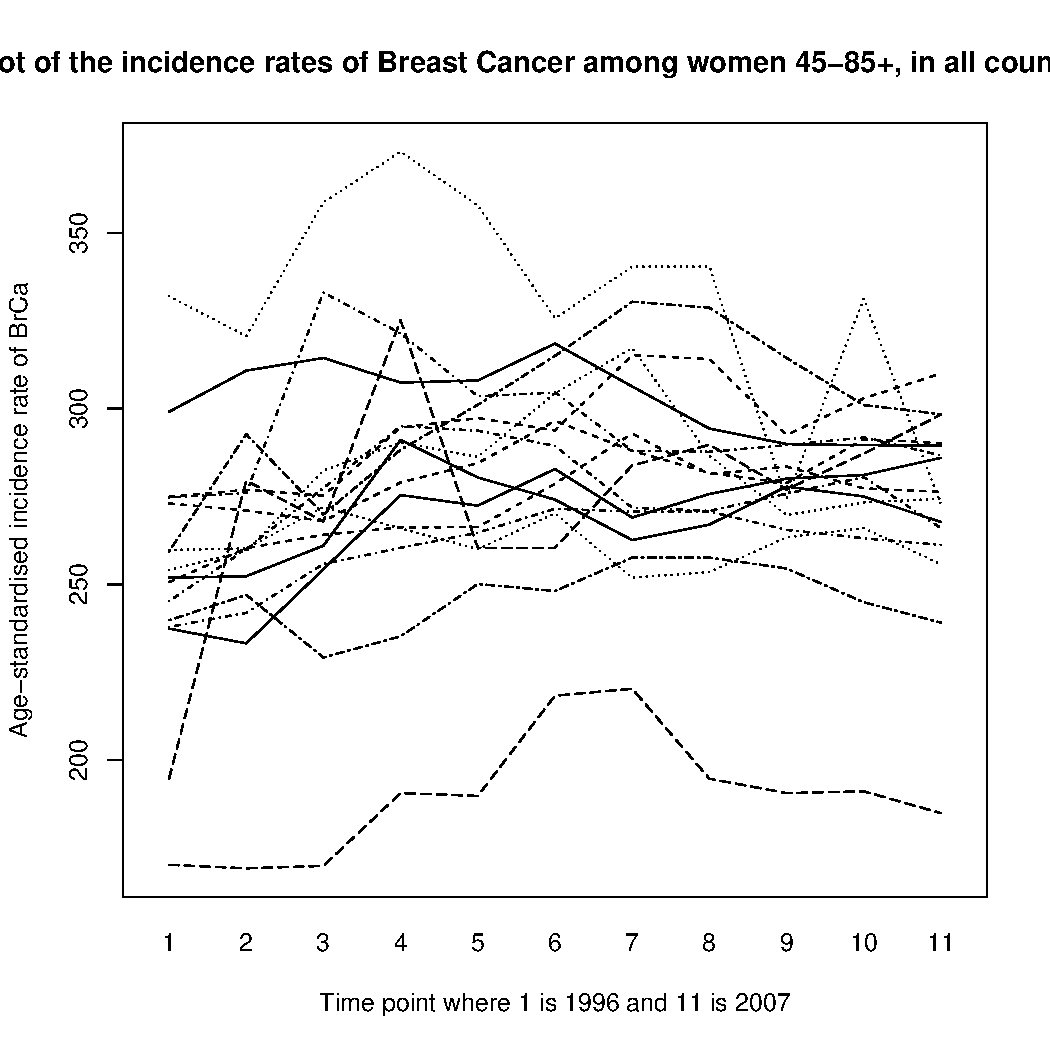
\includegraphics[width=\maxwidth]{figure/sphagettiforall-1} 

\end{knitrout}

\subsubsection*{Figure 1. Age-standardised breast cancer incidence rate among women aged 45-85+ years, all countries, 1996-2007 data}

Visual inspection of this graph suggests two peaks in the plot, one around 2000 and one around 2004-2005 in breast cancer and thereafter there is a drop as po particularly afer the 2001 and then again in 2004. To characteriset this further, we explode this graph into two subgroups, one where peak HRT was reached around 1996-1998 (or at least earlier than 2000 and one where peak HRT uasage was reached after 2000) and examine the two graphs. We found six such countries.

\begin{knitrout}
\definecolor{shadecolor}{rgb}{0.969, 0.969, 0.969}\color{fgcolor}
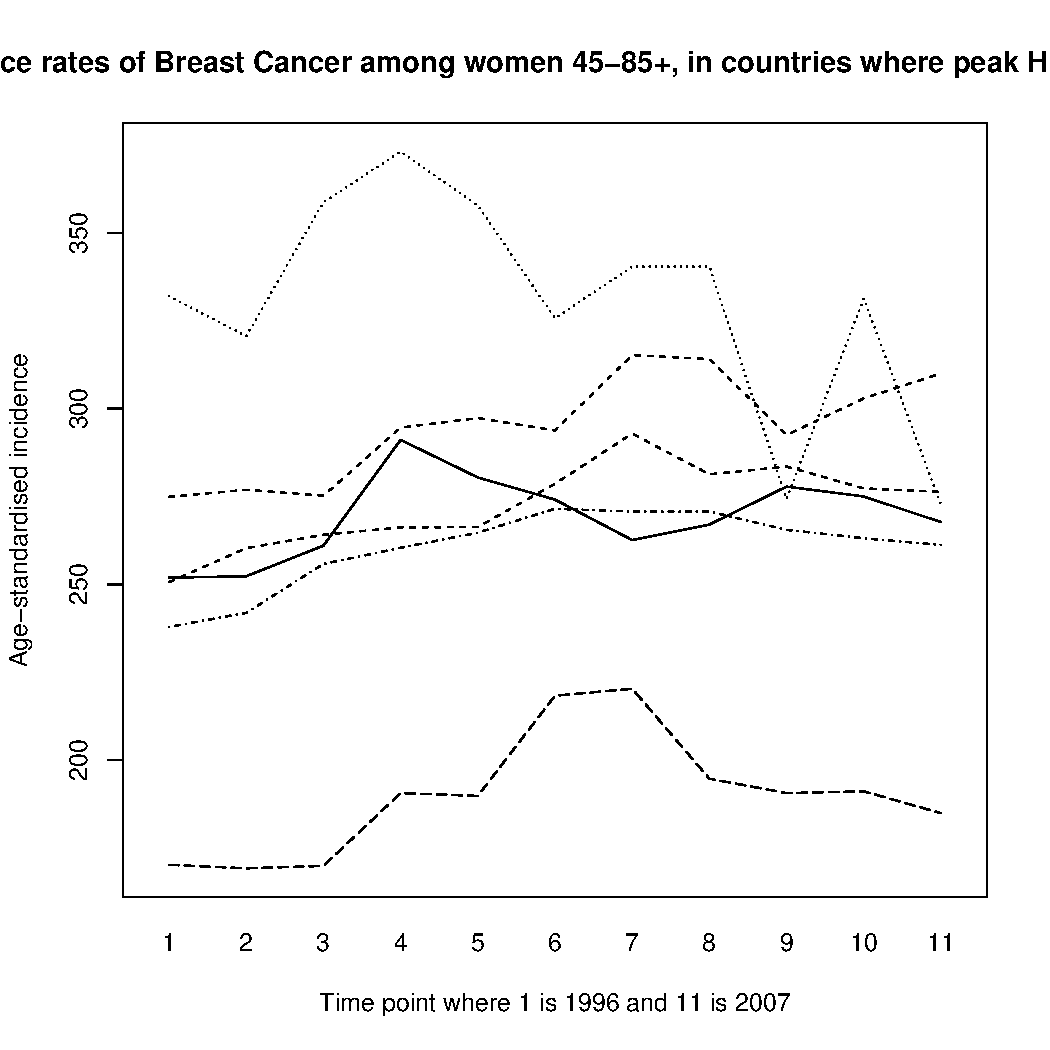
\includegraphics[width=\maxwidth]{figure/sphagettipre2k-1} 

\end{knitrout}

\subsubsection*{Figure 2. Age-standardised breast cancer incidence rate among women aged 45-85+ years, those countries where use of HRT peaked in 1996-1999, 1996-2007 data}

In this graph, we see a reduction in BrCa incidence from 2003 onwards, but a peak in two different time points (??)

Then, we explode another set of graphs where peak HRT use was reached after 2000.

\begin{knitrout}
\definecolor{shadecolor}{rgb}{0.969, 0.969, 0.969}\color{fgcolor}
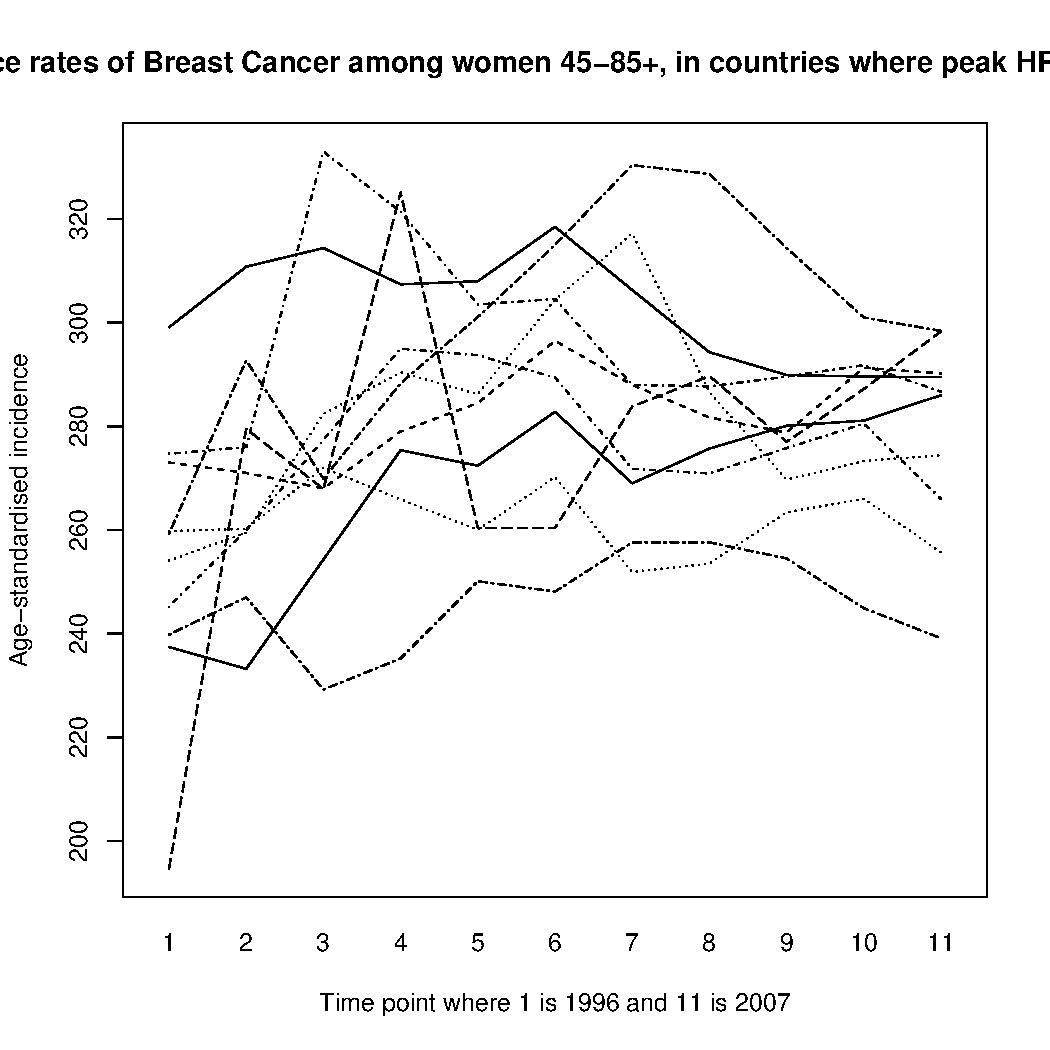
\includegraphics[width=\maxwidth]{figure/peakhrtusepost2k-1} 

\end{knitrout}

\subsubsection*{Figure 3. Age-standardised breast cancer incidence rate among women aged 45-85+ years, those countries where use of HRT peaked in 2000 or afterwards, 1996-2007 data}


Once again, there is a reduction in the BrCa from 2003 onwards. althought the BrCa rates reached a peak in 2002-2003 in most countries almost coeval with the peak in HRT usage.

\end{document}
